%-------------------------------------------------------------------------------
%                            BAB IV
%               		HASIL DAN PEMBAHASAN
%-------------------------------------------------------------------------------

\chapter{HASIL DAN PEMBAHASAN}
	\section{Analisis Kebutuhan Sistem}
		Bagian ini menjelaskan hal-hal yang terkait tentang pengembangan aplikasi sebelum penulisan code sesumber.

		\subsection{Fitur-Fitur Aplikasi}
			Kemampuan menangani sensor-sensor:
			\begin{itemize}
				\item Mampu membaca dan menampilkan suhu yang terbaca pada sensor IQRF,
				\item mampu menyala-matikan relay pada peranti yang diinginkan,
				\item mampu menambah dan mengurangi peranti baru baik IQRF atau XBee,
				\item mampu menjalankan profile tertentu dari kombinasi suhu dan relay atau waktu tertentu.
			\end{itemize}

			Kemampuan menangani pengguna:
			\begin{itemize}
				\item Mengharuskan pengguna untuk memasukkan nama dan kata sandi sebelum masuk ke aplikasi,
				\item dapat menambah atau mengurangi pengguna yang dapat memasuki sistem.
			\end{itemize}

		\subsection{\emph{Use Case Diagram}}
			\begin{figure}[ht!]
			  \centering
			    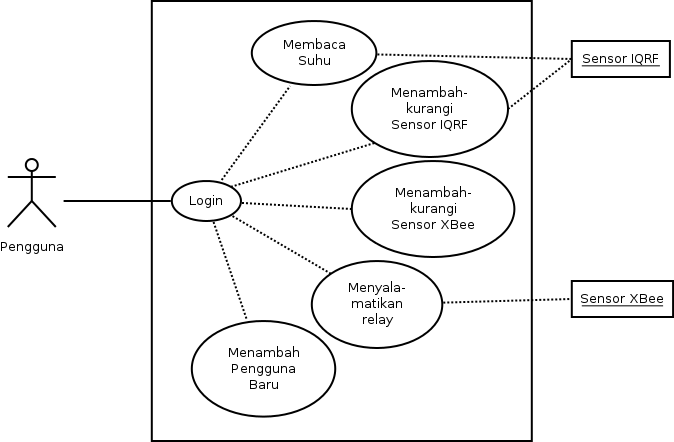
\includegraphics{gambar/usecase}
			    \caption{Diagram \emph{use case} dari penelitian.}
			    \label{usecase}
			\end{figure}

		\subsection{Diagram Arsitektur Sistem}
			\begin{figure}[ht!]
			  \centering
			    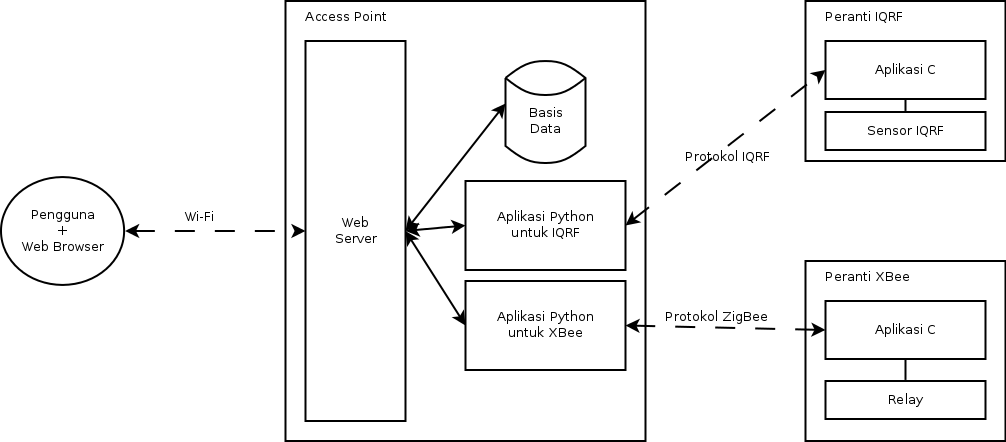
\includegraphics{gambar/system-architecture}
			    \caption{Diagram Arsitektur Sistem.}
			    \label{system-architecture}
			\end{figure}

		\subsection{SDLC}
			\begin{figure}[ht!]
			  \centering
			    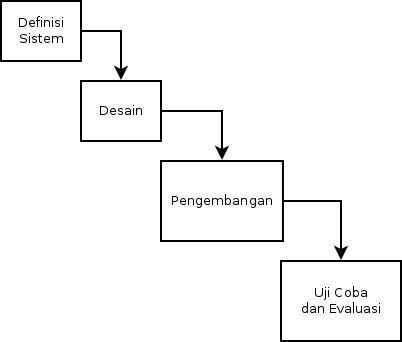
\includegraphics{gambar/sdlc}
			    \caption{Diagram SDLC.}
			    \label{sdlc}
			\end{figure}
	
	\section{Perancangan Aplikasi}
		Bagian ini menjelaskan hal-hal terkait pengembangan aplikasi.

		\subsection{Peta Situs}
			\begin{figure}[ht!]
			  \centering
			    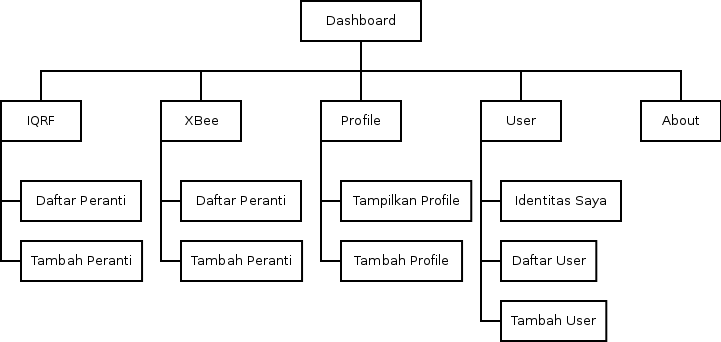
\includegraphics{gambar/sitemap}
			    \caption{Peta situs aplikasi web.}
			    \label{sitemap}
			\end{figure}			

		\subsection{Persiapan Pra Pengembangan Aplikasi}
			\begin{enumerate}
				\item Konfigurasi Router/AP

					Penelitian ini menggunakan AP keluaran TP-LINK seri MR3020. AP jenis ini dipilih karena bentuknya yang kecil sehingga mudah dibawa atau dipindahkan dan kemudahannya untuk dimodifikasi. TP-LINK MR3020 juga terbilang populer di ranah komunitas sistem benam (\emph{embedded device}) sehingga memiliki dukungan yang baik dari pabrikan dan komunitas. 

					Sebelum digunakan, \emph{firmware} bawaan TP-LINK MR3020 harus diganti dengan sistem operasi OpenWRT. Proses penggantian cukup mudah karena hanya memanfaatkan menu \emph{firmware upgrade} dari web admin yang sudah tersedia.	Sistem Operasi OpenWRT yang digunakan adalah Attitude Adjustment versi 12.09 dengan Linux kernel 3.3.8. \emph{Image file} sistem operasi tersebut bisa diunduh secara gratis pada situs \url{www.openwrt.org}.

					Setelah OpenWRT berhasil terinstall, langkah selanjutnya adalah mengimplementasikan \emph{extroot}. \emph{Extroot} dapat memperbesar memori penyimpanan dengan bantuan USB \emph{flash drive}. Langkah yang harus dilakukan pertamakali adalah menginstall perangkat lunak dengan perintah sebagai berikut:
					\begingroup
					    \fontsize{10pt}{12pt}\selectfont
					    \begin{verbatim}
							# opkg update
							# opkg install block-extroot block-hotplug block-mount
					    \end{verbatim}  
					\endgroup

					Kemudian dilanjutkan dengan menyalin isi dari memori internal TP-LINK MR3020 ke USB \emph{flash drive} yang di-\emph{mount} pada direktori /mnt/sda1 dengan perintah:
					\begingroup
					    \fontsize{10pt}{12pt}\selectfont
					    \begin{verbatim}
							# tar -C /overlay -cvf - . | tar -C /mnt/sda1 -xf -
					    \end{verbatim}  
					\endgroup

					Langkah terakhir adalah mengkonfigurasi file /etc/config/fstab dan menyalakan ulang AP. Konfigurasi diganti dengan detil sebagai berikut:
					\begingroup
					    \fontsize{10pt}{12pt}\selectfont
					    \begin{verbatim}
							config mount
						        option target        /mnt
						        option device        /dev/sda1
						        option fstype        ext3
						        option options       rw,sync
						        option enabled       1
						        option enabled_fsck  0
						        option is_rootfs     1
					    \end{verbatim}  
					\endgroup

					Setelah proses implementasi extroot selesai, berarti AP sudah memiliki memori penyimpanan yang cukup (atau mungkin lebih) untuk menginstal aplikasi-aplikasi pendukung lainnya. Penelitian ini menggunakan memori USB 4 Gigabyte.

					Agar TP-LINK MR3020 dapat membaca dan mengirimkan data dari dan ke WSN melalui kanal serial, dibutuhkan Python dan pustaka PySerial yang diinstal dengan perintah:
					\begingroup
					    \fontsize{10pt}{12pt}\selectfont
					    \begin{verbatim}
							# opkg update
							# opkg install python pyserial
					    \end{verbatim}  
					\endgroup

					Sedangkan paket aplikasi `at' digunakan agar AP dapat menjalankan perintah untuk menyala-matikan relay pada waktu tertentu. Namun, sebelum at dapat berjalan, pada router sudah harus tersedia file /var/spool/cron/atjobs/.SEQ dan pemilik dari file tersebut harus diganti menjadi daemon.daemon. Aplikasi `at' diinstall dengan perintah:
					\begingroup
					    \fontsize{10pt}{12pt}\selectfont
					    \begin{verbatim}
							# opkg update && opkg install at
					    \end{verbatim}  
					\endgroup
					
					Langkah selanjutnya adalah instalasi aplikasi pendukung aplikasi berbasis web yang nantinya akan dikembangkan yaitu Web Server, PHP, dan MySQL. Web server yang digunakan adalah yang sudah terinstal pada OpenWRT versi Attitude Adjustment yaitu uHTTPd. Sedangkan PHP dan MySQL harus diinstal dengan perintah:
					\begingroup
					    \fontsize{10pt}{12pt}\selectfont
					    \begin{verbatim}
							# opkg update
							# opkg install php5 php5-cgi mysql
					    \end{verbatim}  
					\endgroup

					Setelah PHP berhasil terinstal, buka file /etc/config/uhttpd dan pastikan baris yang memuat
					\begingroup
					    \fontsize{10pt}{12pt}\selectfont
					    \centering
					    \begin{verbatim}
							list interpreter ".php=/usr/bin/php-cgi"
					    \end{verbatim}  
					\endgroup
					tidak dalam keadaan terkomentar.

					Aplikasi yang terakhir yang harus diinstal adalah SSHFS yang berguna dalam uji coba dan perbaikan aplikasi. SSHFS dapat diinstal dengan perintah:
					\begingroup
					    \fontsize{10pt}{12pt}\selectfont
					    \begin{verbatim}
							# opkg update
							# opkg install sshfs
					    \end{verbatim}  
					\endgroup

					Zona waktu standar pada OpenWRT adalah UTC yang belokasi pada kota Greenwich di Inggris Raya. Agar zona waktu dapat dikonfigurasi sesuai dengan zona waktu kota Yogyakarta, maka isi dari file /etc/config/system harus disesuaikan. Pada file tersebut, zona waktu UTC diganti menjadi WIT-7 atau \emph{Western Indonesian Time}-7.

				\item Konfigurasi Komputer untuk Pengembangan

					Komputer yang digunakan dalam penelitian ini adalah MacBook Pro dengan sistem operasi Mac OSX Mountain Lion. Sedangkan aplikasi yang harus tersedia adalah Sublime Text 3, Arduino for Mac OSX, CoolTerm, Driver FTDI for Mac OSX, IQRF IDE v 2.08 for TR-53B.

					Sublime Text 3 berperan banyak dalam mengedit kode-kode sesumber PHP, C, dan Python.

					Sedangkan proses pengembangan dan pengunduhan aplikasi untuk Arduino sepenuhnya dilakukan dengan Arduino for Mac OSX karena aplikasi tersebut sudah mencakup editor teks dan alat kompilasi.

					Agar komputer dapat membaca kanal serial sehingga dapat melakukan tugas-tugas seperti konfigurasi XBee Radio dan pengujian aplikasi Python, komputer membutuhkan aplikasi CoolTerm. Sebelum aplikaisi ini terinstal, pastikan driver FTDI untuk Mac OSX sudah terinstal, agar komputer dapat mendeteksi XBee yang terhubung melalui USB.

					Walaupun kode sesumber untuk IQRF ditulis dengan bantuan Sublime Text 3, proses kompilasinya dilakukan dengan aplikasi IQRF IDE v 2.08 for TR-53B. Proses pengunduhan file ke IQRF juga dilakukan dengan aplikasi yang sama.

					Semua proses instalasi aplikasi yang dibutuhkan dilakukan dengan prosedur standar dari Mac OSX. Yaitu memperoleh file binary-nya dan kemudian menyalin file tersebut ke direktori Application atau mengikuti prosedur standar dari masing-masing aplikasi.

					Langkah terakhir yang dilakukan adalah memastikan AP dapat mengakses komputer melalui SSH. Pastikan \emph{remote sharing} dalam keadaan tercentang di \emph{System Preference}, \emph{Sharing}. Atau untuk lebih jelasnya dapat melihat pada Gambar \ref{mac-sharing}.

					\begin{figure}[ht!]
					  \centering
					    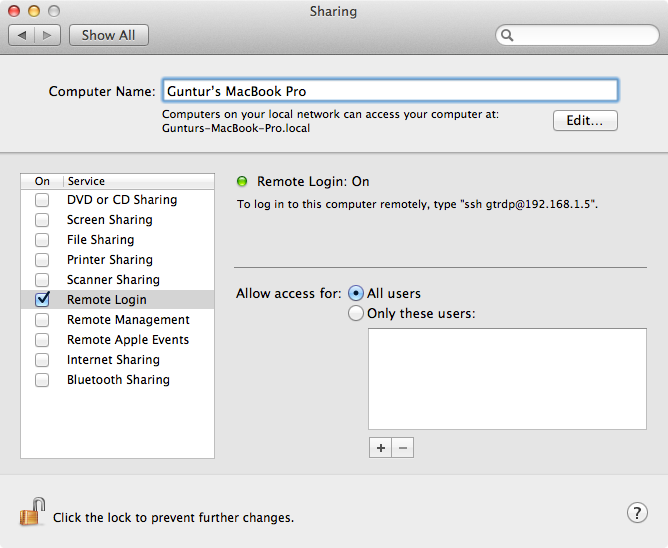
\includegraphics{gambar/mac-sharing}
					    \caption{Konfigurasi SSH pada Mac OSX.}
					    \label{mac-sharing}
					\end{figure}

				\item Peranti XBee

					Setiap peranti XBee yang akan digunakan harus terkonfigurasi terlebih dahulu. Parameter-parameter yang harus terkonfigurasi adalah ATID (alamat dari jaringan/\emph{network ID}), ATMY (alamat peranti itu sendiri), ATDH (\emph{destination address high}), dan ATDL (\emph{destination address low}).

					Proses konfigurasi dilakukan dengan menyambungkan XBee Radio dengan \emph{XBee Explorer USB Board} ke komputer dan menjalankan aplikasi untuk membaca kanal serial, misalnya CoolTerm pada Mac OSX. Setelah CoolTerm dibuka, buka koneksi kanal serial ke XBee dan jalankan perintah dengan format:
					\begingroup
					    \fontsize{10pt}{12pt}\selectfont
					    \begin{verbatim}
					    	+++		#masuk ke AT Mode
							ATID <id jaringan>
							ATMY <alamat dari zigbee>
							ATDH <destination high>
							ATDL <destination low>
							ATWR 	#tulis ke non volatile memory
					    \end{verbatim}  
					\endgroup

					Contoh perintahnya adalah:
					\begingroup
					    \fontsize{10pt}{12pt}\selectfont
					    \begin{verbatim}
							+++		#masuk ke AT Mode
							ATID 1234
							ATMY 5
							ATDH 0
							ATDL 1
							ATWR 	#tulis ke non volatile memory
					    \end{verbatim}  
					\endgroup
			\end{enumerate}

		\subsection{Pengembangan Aplikasi WSN}
			\begin{enumerate}
				\item IQRF

					Peranti IQRF dalam penelitian ini ada dua jenis, begitu pula aplikasi/peranti lunak yang tertanam di dalamnya. Aplikasi tersebut adalah \emph{Sink} dan \emph{Node}. Aplikasi \emph{Sink} akan ditanamkan pada koordinator dari IQRF yang terhubung langsung dengan AP melalui kabel USB dan jumlahnya hanya satu. Sedangkan aplikasi \emph{Node} akan ditanamkan pada sensor-sensor IQRF yang akan saling membentuk jaringan jala (\emph{mesh network}) dan jumlahnya lebih dari satu.

					Aplikasi \emph{Sink} lebih ditekankan pada pembentukan ikatan (\emph{bond}) antara koordinator dan sensor-sensor, pengendalian sensor-sensor, serta pengakuisisian data dari masing-masing sensor.

					Sedangkan aplikasi \emph{Node} lebih bersifat pasif karena hanya akan merespon perintah-perintah yang akan dikirimkan oleh koordinator, seperti pembentukan ikatan dan pembacaan temperatur.

					Data yang akan diakuisisi dari masing-masing sensor adalah temperatur yang terbaca di masing-masing sensor.

					Aplikasi yang digunakan adalah hasil \emph{fork} dari aplikasi iHome yang dikembangkan oleh Sigit B. Wibowo dkk yang fiturnya tidak terbatas hanya pada pembacaan temperatur sekitar.

				\item XBee

					Sama seperti IQRF, peranti XBee terdiri dari dua jenis peranti, yaitu koordnator dan sensor-sensor. Koordinator bertugas menyala dan matikan relay-relay yang terdapat di masing-masing sensor sesuai permintaan pengguna.

					Koordinator tersusun atas \emph{XBee 802.15.4 Radios (Series 1)} yang tertanam pada \emph{XBee Explorer USB Board} dan terkoneksi langsung dengan AP dengan kabel USB.

					Sedangkan sensornya terdiri dari tiga bagian, yaitu \emph{XBee 802.15.4 Radios (Series 1)}, \emph{2 channel Relay Shield For Arduino (With XBee/BTBee interface)}, dan Arduino Uno. Ketiga bagian tersebut saling terhubung dengan pin-pin yang tersedia.

					XBee pada hakikatnya hanya sebatas peranti komunikasi antara AP dengan relay-relay yang tersedia, sehingga pemrograman teletak pada masing-masing Arduino pada relay. Bahasa yang digunakan adalah bahasa C (Arduino). Aplikasi yang dikembangkan akan menunggu perintah dari AP untuk menyala dan matikan relay.

			\end{enumerate}

		\subsection{Pengembangan Aplikasi Python}
			Aplikasi Python adalah jantung dari penelitian ini karena menghubungkan aplikasi berbasis web dengan peranti-peranti IQRF dan XBee.

			Aplikasi terdiri dari tiga bagian.

			\begin{enumerate}
				\item IQRF

					Aplikasi Python IQRF memiliki kemampuan untuk melakukan \emph{bonding} antara koordinator dan sensor, dan pembacaan temperatur pada sensor dengan ID tertentu.

					Diagram alir dari aplikasi berikut dapat dilihat pada Gambar \ref{python-iqrf}.

					\begin{figure}[ht!]
					  \centering
					    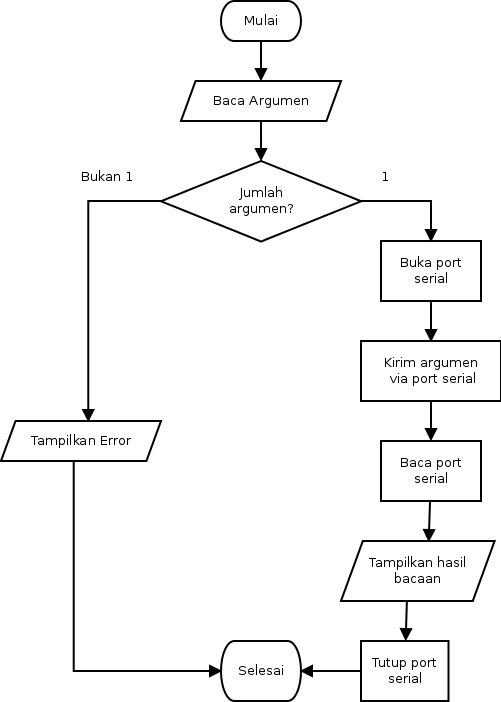
\includegraphics{gambar/python-iqrf}
					    \caption{Diagram alir aplikasi Python untuk IQRF.}
					    \label{python-iqrf}
					\end{figure}

					Aplikasi dijalankan dengan menjalankan format perintah berikut pada \emph{terminal console}:
					\begingroup
					    \fontsize{10pt}{12pt}\selectfont
					    \begin{verbatim}
					    	$ python iqrf.py <perintah><ID node>
					    \end{verbatim}  
					\endgroup

					Aplikasi ini berjalan dalam bentuk CLI dan membutuhkan satu parameter, yaitu perintah yang langsung disambung dengan ID node tanpa spasi. Perintah yang tersedia yaitu membaca gemperatur pada node ID tertentu (g), \emph{bonding} node ID tertentu (b), \emph{unbonding} node ID tertentu (u).

					Sehingga contoh penggunaan aplikasi pada \emph{terminal console}:
					\begingroup
					    \fontsize{10pt}{12pt}\selectfont
					    \begin{verbatim}
					    	$ python iqrf.py g3
					    \end{verbatim}  
					\endgroup
					Perintah di atas adalah perintah untuk membaca temperatur pada node ID 3.

				\item XBee

					Aplikasi Python XBee memiliki kemampuan untuk menyala dan matikan relay pada peranti tertentu dan membaca status relay pada peranti tertentu, apakah relay tersebut sedang menyala atau mati.

					Diagram alir dari aplikasi berikut dapat dilihat pada Gambar \ref{python-xbee}.

					\begin{figure}[ht!]
					  \centering
					    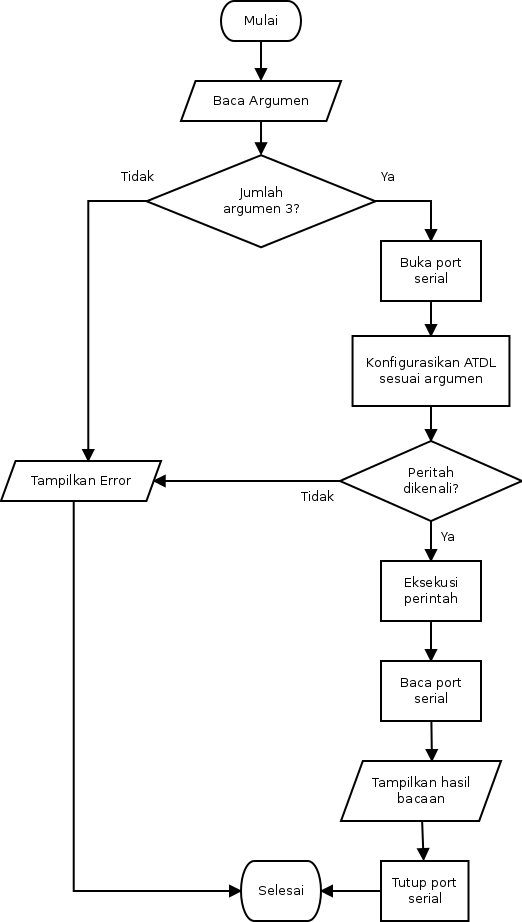
\includegraphics{gambar/python-xbee}
					    \caption{Diagram alir aplikasi Python untuk menangani peranti XBee.}
					    \label{python-xbee}
					\end{figure}

					Aplikasi dijalankan dengan menjalankan format perintah berikut pada \emph{terminal console}:
					\begingroup
					    \fontsize{10pt}{12pt}\selectfont
					    \begin{verbatim}
					    	$ python xbee.py <perintah> <ATMY peranti> <ID relay>
					    \end{verbatim}  
					\endgroup

					Aplikasi ini berjalan dalam bentuk CLI dan membutuhkan tiga parameter, yaitu perintah, alamat peranti (ATMY), dan ID relay (terdapat dua relay di tiap peranti). Perintah yang tersedia yaitu menyalakan relay, `on', mematikan relay, `off', dan membaca status relay, `status'.

					Sehingga contoh penggunaan aplikasi pada \emph{terminal console}:
					\begingroup
					    \fontsize{10pt}{12pt}\selectfont
					    \begin{verbatim}
					    	$ python iqrf.py status 2 1
					    \end{verbatim}  
					\endgroup
					Perintah di atas akan membaca status (on/off) dari relay 1 pada peranti dengan alamat (ATMY) 2 dan menampilkannya pada layar dalam karakter `H' (menyala) atau `L' (mati).

				\item Profile

					Aplikasi ini memanfaatkan aplikasi \emph{at} pada Linux yang dapat menjalankan perintah tertentu di \emph{terminal console} pada waktu tertentu. Dengan aplikasi ini, pengguna dapat menyala-matikan relay pada waktu tertentu. Jika hal ini dikombinasikan dengan bacaan temperatur dari sensor IQRF, maka pengguna dapat menyala-matikan relay tertentu pada saat temperatur pada sensor IQRF node tertentu mencapai suhu tertentu, dan juga bisa hanya terjadi saat waktu tertentu.

					Diagram alir dari aplikasi berikut dapat dilihat pada Gambar \ref{python-profile}.

					\begin{figure}[ht!]
					  \centering
					    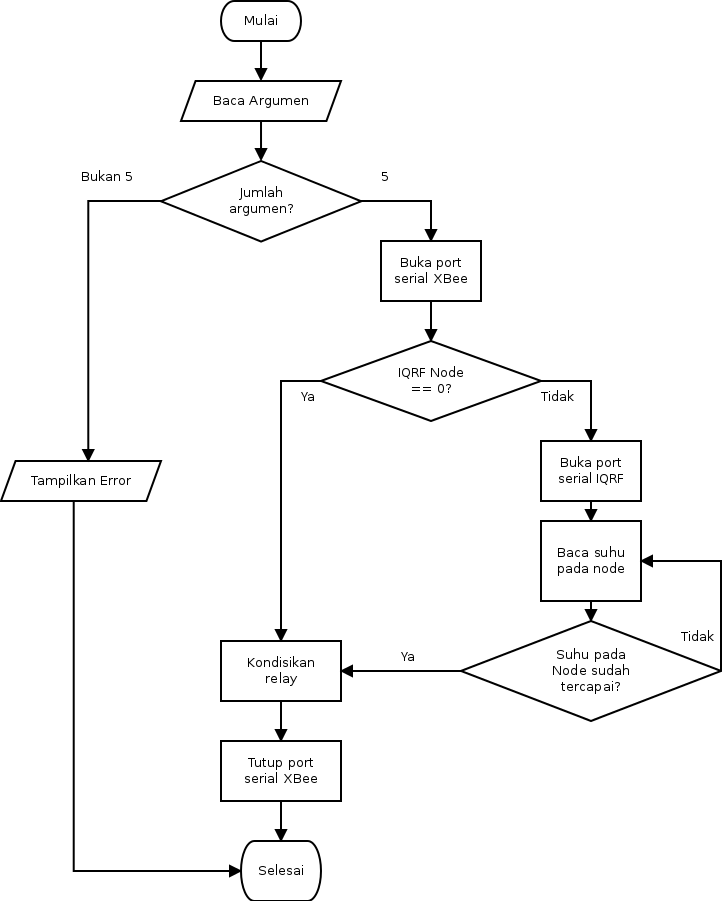
\includegraphics{gambar/python-profile}
					    \caption{Diagram alir aplikasi Python untuk menyala-matikan lampu pada kondisi tertentu.}
					    \label{python-profile}
					\end{figure}

			\end{enumerate}

		\subsection{Pengembangan Aplikasi Berbasis Web}
			Aplikasi web untuk mengendalikan sensor-sensor IQRF dan XBee dibangun dengan PHP dan basis data MySQL. Aplikasi ini dibangun tanpa menggunakan \emph{framework} karena aplikasi ini tergolong tidak terlalu rumit, aplikasi ini hanya memliki lima halaman utama seperti terlihat pada sitemap Gambar \ref{sitemap}. Penggunaan \emph{framework} juga akan memakan sumber daya komputasi sedikit lebih banyak, padahal aplikasi ini akan diimplementasikan pada sebuah AP yang memiliki tingkat komputasi yang rendah.

			Antarmuka yang dikembangkan adalah hasil \emph{fork} dari \emph{template} halaman administrator buatan Vince G. Antarmuka ditulis menggunakan HTML5 dan CSS3, dengan tambahan pemrograman JavaScript pada sisi klien agar menambah interaktivitas. Pustaka Bootstrap digunakan untuk membuat halaman web menjadi responsif, sehingga dapat menyesuaikan diri secara otomatis sesuai dengan ukuran layar. Pustaka jQuery digunakan untuk membantu pemrograman di sisi klien.

			

			Dikembangkan dengan pustaka Bootstrap.
			Diagram alir menambah peranti IQRF:

			\begin{figure}[ht!]
			  \centering
			    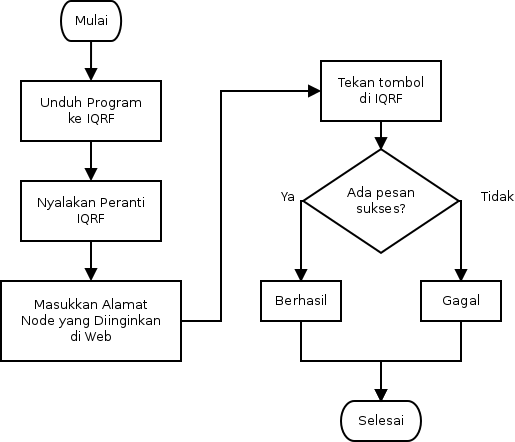
\includegraphics{gambar/add-iqrf}
			    \caption{Diagram Alir Penambahan Peranti IQRF ke Aplikasi.}
			    \label{add-iqrf}
			\end{figure}

			Diagram alir menambah peranti XBee:

			\begin{figure}[ht!]
			  \centering
			    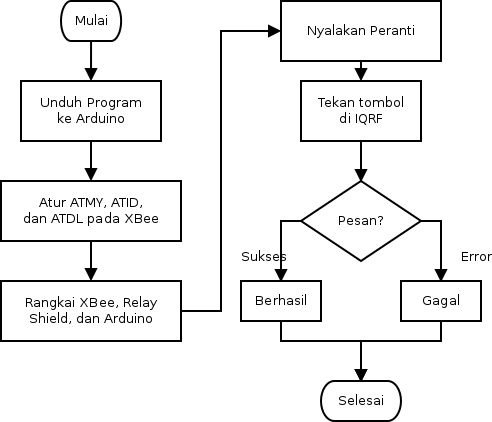
\includegraphics{gambar/add-xbee}
			    \caption{Diagram Alir Penambahan Peranti XBee ke Aplikasi.}
			    \label{add-xbee}
			\end{figure}


			ERD
		\subsection{Evaluasi dan Perbaikan}
			Peranan SSHFS.

		\subsection{\emph{Screenshot} Aplikasi}

			Tampilkan responsif untuk beberapa halaman.

		\subsection{Kode Sesumber}
			Kode sesumber dapat diperoleh pada situs GitHub dengan alamat URL \url{https://github.com/gtrdp/wsn-ip-interoperability}.


	\section{Analisis Unjuk Kerja Aplikasi}
		Bagian ini menjelaskan hal-hal terkait instalasi aplikasi ke kondisi sesungguhnya, hasil uji coba, masalah, dan penyelesaian.

		\subsection{Hasil Akhir Perangkat Keras}
		\subsection{Instalasi Aplikasi dan Perangkat Keras}
		\subsection{Hasil Uji Coba Aplikasi}
		\subsection{Masalah dan Penyelesaian}
